\documentclass[11pt,a4paper,parskip=half]{scrartcl}
\usepackage[T1]{fontenc}
\usepackage[utf8]{inputenc}
%\usepackage{tgpagella}
\usepackage{tgheros} % TeX Gyre Heros (sans-serif for headings)
\usepackage[bitstream-charter]{mathdesign} % Bitstream Charter (for text)
\usepackage[bf,sf]{titlesec} % not needed atm?
\usepackage[protrusion=true,expansion=true]{microtype} % "beautification"
\usepackage{geometry}
\geometry{left=2.5cm,right=2.5cm,bottom=4cm,top=3cm}

\usepackage{caption}
\usepackage{subcaption}
\usepackage{etoolbox}
\usepackage{fancyhdr}
\usepackage{enumerate}
\usepackage{booktabs}
\usepackage[usenames,dvipsnames]{xcolor}
\usepackage{wrapfig}
\usepackage{url}
%\usepackage{gb4e}
\usepackage{covington}
\usepackage{ngerman}
\usepackage[style=1]{mdframed}

\newtoggle{usenorm}
\toggletrue{usenorm}

\begin{document}

\newcommand{\mmb}{Marcel Bollmann ({\small\url{bollmann@linguistics.rub.de}})}
\newcommand{\trans}[1]{"`{\small\texttt{#1}}"'}

%%%%%%%%%%%%%%%%%%%%%%%%%%%%%%%%%%%%%%%%%%%%%%%%%%
%%%% DEFINITION OF BOX ENVIRONMENTS %%%%%%%%%%%%%%
%%%%%%%%%%%%%%%%%%%%%%%%%%%%%%%%%%%%%%%%%%%%%%%%%%

\newenvironment{infobox}[1]{
  \begin{mdframed}[linewidth=1,leftmargin=20,rightmargin=20,%
    backgroundcolor=Yellow!50,linecolor=GreenYellow,%
    splittopskip=\topskip,skipbelow=0.5\baselineskip,%
    skipabove=\baselineskip,%
    roundcorner=6pt,%
    innerleftmargin=6pt,innerrightmargin=6pt,%
    innerbottommargin=.85\baselineskip,innertopmargin=0pt]
    \textbf{#1}\\
}{
  \end{mdframed}
}

\newenvironment{alertbox}[1]{
  \begin{mdframed}[linewidth=1,leftmargin=20,rightmargin=20,%
    backgroundcolor=Red!45,linecolor=Sepia,%
    splittopskip=\topskip,skipbelow=0.5\baselineskip,%
    skipabove=\baselineskip,%
    roundcorner=6pt,%
    innerleftmargin=6pt,innerrightmargin=6pt,%
    innerbottommargin=.85\baselineskip,innertopmargin=0pt]
    \textbf{#1}\\
}{
  \end{mdframed}
}

%%%%%%%%%%%%%%%%%%%%%%%%%%%%%%%%%%%%%%%%%%%%%%%%%%
%%%% TITLE AND PAGE STYLES %%%%%%%%%%%%%%%%%%%%%%%
%%%%%%%%%%%%%%%%%%%%%%%%%%%%%%%%%%%%%%%%%%%%%%%%%%

\pagestyle{fancy}
\lhead{\emph{CorA Benutzerhandbuch}}
%\rhead{108004242751 $\cdot$ Bollmann}

%\originalTeX

\title{CorA (Corpus Annotator)\\Benutzerhandbuch}
\subtitle{Version 1.0} \author{Marcel
  Bollmann\\\url{bollmann@linguistics.rub.de}\\Sprachwissenschaftliches
  Institut\\Ruhr-Universität Bochum} \date{\today}
\maketitle

%\setcounter{page}{1}
\tableofcontents
\newpage

%%%%%%%%%%%%%%%%%%%%%%%%%%%%%%%%%%%%%%%%%%%%%%%%%%
%%%% CONTENT %%%%%%%%%%%%%%%%%%%%%%%%%%%%%%%%%%%%%
%%%%%%%%%%%%%%%%%%%%%%%%%%%%%%%%%%%%%%%%%%%%%%%%%%

\section{Allgemeines}

CorA ist ein web-basiertes Programm zur Annotation von Korpora.  Die
aktuelle Adresse~(URL) von CorA lautet:

\begin{quote}
  \url{http://smokehead.linguistics.rub.de/cora/}
\end{quote}

Wir empfehlen die Verwendung einer aktuellen Version von Google
Chrome\footnote{\url{http://www.google.com/chrome/}} (bzw.\ Chromium)
oder Mozilla Firefox\footnote{\url{http://www.mozilla.com/}}.
JavaScript darf nicht deaktiviert sein.  CorA funktioniert
möglicherweise auch mit anderen Browsern, jedoch wird das Tool von uns
nur mit den genannten Browsern getestet.

\begin{alertbox}{Wichtig!}
  Die Benutzung von CorA erfordert eine ständige Internetverbindung.
  Es ist nicht möglich, das Tool offline zu benutzen.  Wenn Sie
  während der Bearbeitung eines Dokuments länger als 30~Minuten
  offline sind, kann ein Datenverlust nicht ausgeschlossen werden.
\end{alertbox}

Bitte öffnen Sie CorA \textbf{nicht} gleichzeitig in mehreren
Browserfenstern auf demselben Rechner, und loggen Sie sich
\textbf{nicht} gleichzeitig mit demselben Benutzerkonto auf mehreren
Rechnern ein.  Dies kann zu unvorhergesehenem Verhalten führen, da
CorA hierfür nicht ausgelegt ist.

\subsection{Benutzername und Passwort}

Bevor Sie CorA benutzen können, müssen Sie sich mit Benutzernamen und
Passwort anmelden.  Falls ein neues Benutzerkonto angelegt werden
soll, oder Sie Ihr Passwort vergessen haben, wenden Sie sich bitte
direkt an \mmb{}.

Ihr \textbf{Passwort ändern} können Sie hingegen direkt in CorA:
hierzu loggen Sie sich zunächst ein, wechseln zum Reiter
"`Einstellungen"' und klicken dort auf die Schaltfläche "`Passwort
ändern\ldots"'.  Wenn Sie sich zum ersten Mal einloggen, sollten Sie
als erstes unbedingt Ihr Passwort ändern!

\newpage
\section{Dateiverwaltung}
\label{sec:datei}

\begin{figure}[!b]
  \centering
  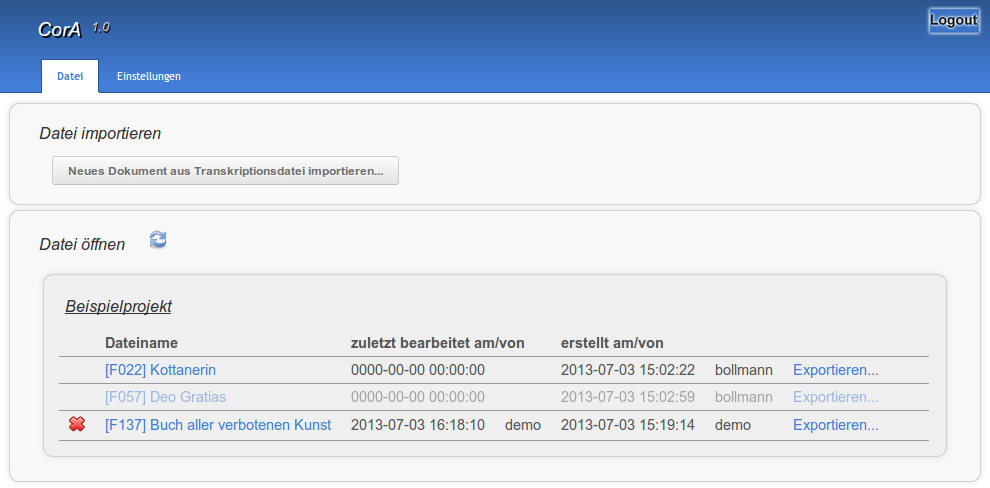
\includegraphics[width=\linewidth]{img/datei.png}
  \caption{Dateien verwalten}
  \label{fig:datei}
\end{figure}

Nach der Anmeldung in CorA wird zunächst der Reiter "`Datei"'
angezeigt.  Abbildung~\ref{fig:datei} zeigt einen Beispiel-Screenshot,
der im Folgenden näher erläutert wird.

% Dateien in CorA sind immer \emph{Projekten} zugeordnet.  In
% Abbildung~\ref{sec:datei} gibt es nur ein Projekt (mit Namen
% "`Beispielprojekt"'), welches drei Texte enthält.

\subsection{Öffnen einer Datei}

Klicken Sie einfach auf einen Dateinamen, um die entsprechende Datei
zum Annotieren zu öffnen.  Nun öffnet sich automatisch das
Editor-Fenster (s.\ Abschnitt~\ref{sec:editor}).

Dateinamen, die in der Liste \textbf{leicht ausgegraut} erscheinen
(wie z.B.\ "`Deo Gratias"' in Abbildung~\ref{fig:datei}), sind bereits
von einem anderen Nutzer geöffnet.  Eine Datei kann immer \textbf{nur
  von einem Nutzer gleichzeitig} geöffnet sein!  Klicken Sie den
Dateinamen an, um zu erfahren, wer die Datei aktuell geöffnet hat.
Die Datei kann erst wieder von jemand anderem geöffnet werden, wenn
dieser Nutzer entweder
\begin{itemize}
\item die Datei über den Knopf "`Datei schließen"' schließt,
\item sich aus CorA ausloggt (über den Knopf "`Logout"' oben rechts),
  oder
\item länger als 30~Minuten nicht mehr online gewesen ist.
\end{itemize}

Durch Klicken auf das
Symbol 
\includegraphics[height=0.9\baselineskip]{img/view-refresh.png}
wird die Dateiliste aktualisiert.


\subsection{Importieren von Transkriptionen}
\label{sec:datei-import}

\begin{figure}
  \centering
  \begin{subfigure}[b]{0.45\textwidth}
    \centering
    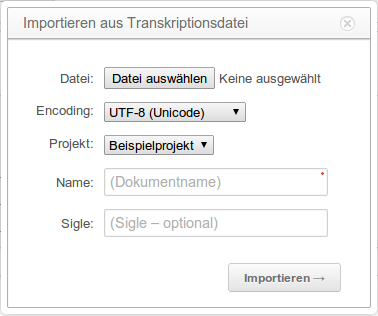
\includegraphics[width=\textwidth]{img/import-trans.png}
    \caption{Vor dem Import}
    \label{fig:import-dialog}
  \end{subfigure}
  \hfill
  \begin{subfigure}[b]{0.45\textwidth}
    \centering
    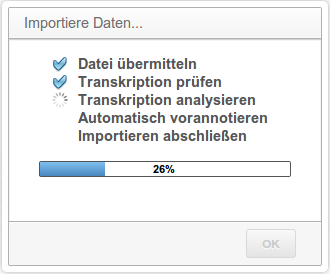
\includegraphics[width=\textwidth]{img/import-trans-progress.png}
    \caption{Während des Imports}
    \label{fig:import-progress}
  \end{subfigure}
  \caption{Importieren einer Datei}
  \label{fig:import}
\end{figure}

Um eine neue Datei hinzuzufügen, klicken Sie auf den Knopf "`Neues
Dokument aus Transkriptionsdatei importieren\ldots"' (s.\
Abbildung~\ref{fig:datei}).

Es öffnet sich ein Fenster ähnlich wie in
Abbildung~\ref{fig:import-dialog}.  Wählen Sie hier die \textbf{Datei}
aus, die Sie hochladen möchten, und geben Sie an in welchem
\textbf{Encoding} die Datei gespeichert wurde.  Stellen Sie ggf.\
sicher, dass das richtige \textbf{Projekt} ausgewählt ist (z.B.\
"`Referenzkorpus Frühneuhochdeutsch"').  Sie müssen außerdem
\textbf{Name} und \textbf{Sigle} des Dokuments angeben, unter denen es
in CorA geführt werden soll.

Der Import startet nach Klick auf "`Importieren"'.  Es öffnet sich ein
neues Fenster, welches den Fortschritt des Importvorgangs anzeigt
(Abbildung~\ref{fig:import-progress}).  Je nach Umfang der Datei kann
der Import \textbf{ca.\ 10~bis 15~Minuten} in Anspruch nehmen.  Bitte
schließen Sie das Browserfenster in dieser Zeit nicht!\footnote{Wenn
  Sie das Browserfenster während eines laufenden Imports schließen,
  läuft der Import trotzdem weiter.  Sie können allerdings
  möglicherweise auftretende Fehlermeldungen nicht mehr sehen, und
  eventuell auch nicht mehr auf CorA zugreifen, bevor der Import
  beendet ist.}  Arbeiten Sie auch nicht in einem anderen Fenster mit
CorA weiter!

\begin{infobox}{Fehlermeldungen}
  Während des Imports können u.U.\ auch Fehlermeldungen auftreten,
  z.B.\ wenn das Check-Skript noch Fehler in der Transkription
  bemängelt oder wenn das Encoding falsch angegeben wurde.  Falls
  jedoch andere Fehlermeldungen mit für Sie unverständlichem Inhalt
  auftreten sollten, melden Sie uns diese und beachten bitte unbedingt
  auch die Hinweise in Abschnitt~\ref{sec:error}, die wir extra für
  diesen Fall zusammengestellt haben!
\end{infobox}

% Während des Imports können auch \textbf{Fehlermeldungen} auftreten.
% Dies kommt z.B.\ vor, wenn das Check-Skript noch Fehler in der
% Transkription bemängelt, oder wenn das Encoding falsch angegeben
% wurde.  Falls jedoch andere Fehlermeldungen auftreten sollten, die Sie
% sich nicht erklären können, melden Sie sich bitte bei uns!  Beachten
% Sie dazu unbedingt auch die Hinweise in Abschnitt~\ref{sec:error}, die
% wir extra für diesen Fall zusammengestellt haben.

\subsection{Exportieren}
\label{sec:datei-export}

Jede Datei in der Dateiliste besitzt am Ende der Zeile einen Link
"`Exportieren\ldots"' (s.\ Abbildung~\ref{fig:datei}).  Diese
Funktionalität ist in der aktuellen CorA-Version jedoch noch nicht
implementiert und wird zu einem späteren Zeitpunkt nachgeliefert.

\subsection{Löschen}
\label{sec:datei-delete}

Dateien können durch Klick auf das rote
Kreuz 
\includegraphics[height=0.8\baselineskip]{img/delete.png} vor
dem jeweiligen Dateinamen (s.\ Abbildung~\ref{fig:datei}) wieder gelöscht werden.  Das Löschen von
Dateien ist endgültig und \textbf{kann nicht rückgängig gemacht
  werden!}  Es erscheint daher eine entsprechende Warnung, die
bestätigt werden muss, bevor die Datei tatsächlich gelöscht wird.

Nur der Benutzer, der die Datei importiert hat, kann sie auch wieder
löschen.  Allen anderen Nutzern wird das entsprechende Symbol gar
nicht erst angezeigt.

\newpage
\section{Das Editor-Fenster}
\label{sec:editor}

\begin{figure}[!b]
  \centering
  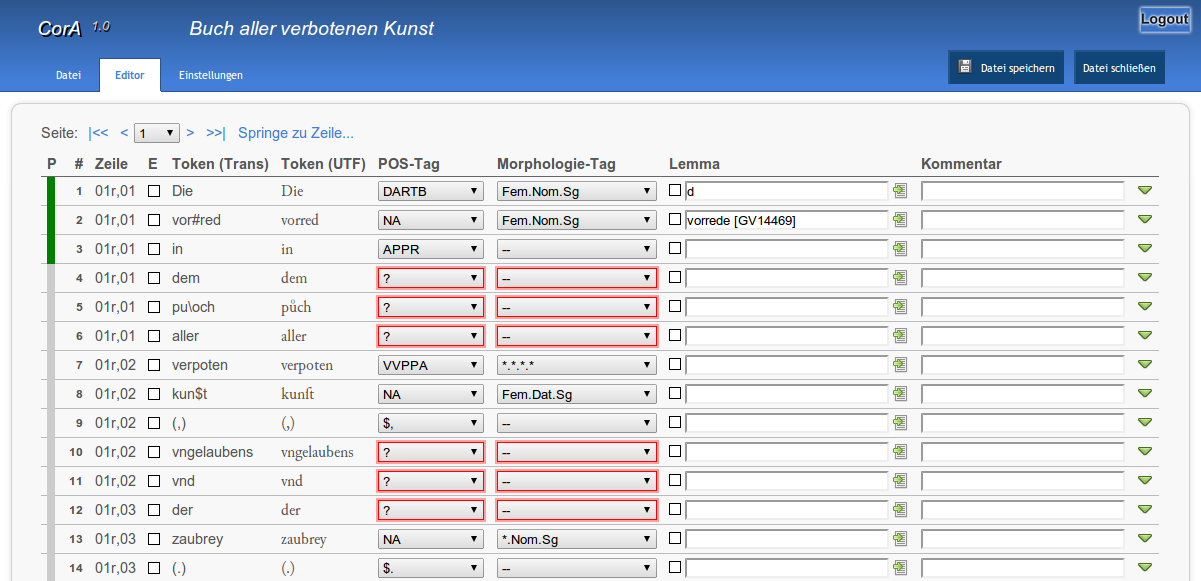
\includegraphics[width=\linewidth]{img/editor.png}
  \caption{Das Editor-Fenster}
  \label{fig:editor}
\end{figure}

Der Editor ist der zentrale Bestandteil von CorA.  Er öffnet sich
automatisch, wenn eine Datei geöffnet wird, bzw.\ durch Klick auf den
Reiter "`Editor"' am oberen Bildschirmrand.
Abbildung~\ref{fig:editor} zeigt einen Beispiel-Screenshot.

\subsection{Navigationsleiste}

Am oberen Rand des Editors befindet sich eine Leiste, mit der
innerhalb des Dokuments navigiert werden kann:

\begin{center}
  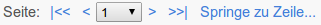
\includegraphics[height=15px]{img/navigation.png}
\end{center}

\begin{itemize}
\item "`|<{}<"' bzw. "`|>{}>"' springt zur ersten bzw. letzten Seite
  des Dokuments
\item "`<"' bzw. "`>"' blättert eine Seite zurück bzw. vor
\item Die Dropdown-Box in der Mitte zeigt die momentane Seitenzahl an;
  Auswählen einer anderen Seitenzahl springt zur entsprechenden Seite.
\item Klicken auf "`Springe zu Zeile\ldots{}"' öffnet ein Fenster, wo
  eine Zeilennummer eingegeben werden kann; der Editor springt dann
  auf die Seite, die die entsprechende Zeilennummer enthält.
\end{itemize}

Zeilen- und Seitenzahlen beziehen sich dabei immer auf die Darstellung
im Editor, \textbf{nicht} auf Zeilen bzw.\ Seiten in der
Transkription!  Funktionen zum Navigieren anhand der Nummerierung in
der Original-Transkription sind momentan noch nicht implementiert.

\subsection{Spalten im Editor}

Wortformen im CorA-Editor werden immer zeilenweise angezeigt, wobei
jede Zeile ein Token nach moderner Tokenisierung enthält.  Im
Folgenden werden Bedeutung und Funktionsweise der einzelnen Spalten
erläutert.

\subsubsection{Fortschrittsbalken (P)}

\begin{wrapfigure}{r}{0.1\textwidth}
  \begin{center}\vspace{-2em}
    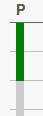
\includegraphics[width=0.05\textwidth]{img/progress.png}
  \end{center}
\end{wrapfigure}

Der Fortschrittsbalken soll anzeigen, bis zu welchem Punkt eine Datei
bereits bearbeitet worden ist.  Eine \textbf{grüne} Markierung zeigt
den bereits bearbeiteten Bereich an, während der Balken ansonsten
\textbf{grau} hinterlegt ist.

Diese Markierung erfüllt derzeit folgende Funktionen:
\begin{itemize}
\item Wenn eine Datei geöffnet wird, springt der Editor automatisch an
  die Stelle, wo der Fortschrittsbalken endet.
\item Die automatische Lernfunktion lernt nur aus den Daten, die
  bereits grün markiert sind. (noch nicht implementiert)
\end{itemize}

Wird eine Annotation an einem Token geändert, verlängert sich der
Fortschrittsbalken ggf.\ automatisch bis zu diesem Punkt.  Bedenken
Sie dies insbesondere, falls Sie einmal an eine spätere Stelle im Text
springen, um dort eine Annotation zu ändern!  Sie müssen sich in
diesem Fall merken, an welchem Punkt Sie zuvor gewesen sind, da die
Fortschrittsanzeige sich automatisch verlängert.

Durch Klick auf den Fortschrittsbalken kann dieser allerdings bei
Bedarf auch manuell eingestellt werden: Klick auf einen grünen Bereich
verkürzt den Balken bis zu diesem Punkt, Klick auf einen grauen
Bereich verlängert ihn entsprechend.


\subsubsection{Nummerierung}

\begin{wrapfigure}{r}{0.12\textwidth}
  \begin{center}\vspace{-2em}
    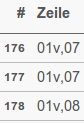
\includegraphics[width=0.1\textwidth]{img/zeile.png}
  \end{center}
\end{wrapfigure}

Zwei verschiedene Zeilennummern werden angezeigt:
\begin{enumerate}
\item Die interne Nummerierung (Spalte "`\#"') ist eine fortlaufende
  Zählung aller Token; über den Link "`Springe zu Zeile\ldots"' in der
  Navigationsleiste kann z.B.\ direkt zu einer bestimmten Zeilennummer
  gesprungen werden.
\item Die Spalte "`Zeile"' gibt die Zeilennummer in der
  Original-Transkription an. (In Einzelfällen, wenn ein Wort sich über
  mehrere Zeilen erstreckt, kann diese Angabe ungenau sein. Dies ist
  eine bekannte Einschränkung.)
\end{enumerate}

\newpage %% HACK
\subsubsection{Markierung von Problemfällen (E)}

\begin{wrapfigure}{r}{0.1\textwidth}
  \begin{center}\vspace{-2em}
    
\includegraphics[width=0.031\textwidth]{img/error.png}
  \end{center}
\end{wrapfigure}

Die Spalte "`E"' (ursprünglich für "`Error"') enthält eine Checkbox,
in der durch Anklicken eine rote Markierung gesetzt bzw.\ entfernt
werden kann.  Diese Markierung ist lediglich eine Hilfe für den
Bearbeiter und hat intern keine weitere Funktion.  Sie kann z.B.\
benutzt werden, um Fehler oder Problemfälle zu markieren, die später
noch einmal angesehen werden müssen.

Es wird in Zukunft eine Suchfunktion geben, mit der gezielt nach
derart markierten Token gesucht werden kann.

\subsubsection{Token}

Es gibt zwei verschiedene Darstellungen der Wortformen, die annotiert
werden sollen: \textbf{Token~(Trans)} zeigt die
Original-Transkription, während \textbf{Token~(UTF)} eine
Unicode-Darstellung der Transkriptionszeichen enthält.  Es ist
möglich, den Editor so anzupassen, dass nur eine der beiden Formen
dargestellt wird -- siehe dazu Abschnitt~\ref{sec:anpassen}.

\subsubsection{POS- und Morphologie-Tags}

\begin{wrapfigure}{r}{0.35\textwidth}
  \begin{center}\vspace{-2em}
    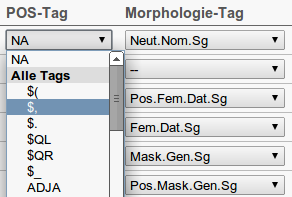
\includegraphics[width=0.3\textwidth]{img/pos.png}
  \end{center}
\end{wrapfigure}

Die Wortarten-Annotation in CorA erfolgt in zwei Schritten: zunächst
sollte über die entsprechende Dropdown-Box ein \textbf{POS-Tag}
ausgewählt werden; anschließend kann in der Spalte
\textbf{Morphologie-Tag} eine Kombination von morphologischen Angaben
ausgewählt werden.

Die Auswahlmöglichkeiten bei den Morphologie-Tags sind dabei
\textbf{abhängig vom gewählten POS-Tag}.  Falls der POS-Tag geändert
wird, und der aktuell selektierte Morphologie-Tag keine zulässige
Auswahl mehr für den neuen POS-Tag ist, so ändert CorA den
Morphologie-Tag \textbf{automatisch} auf einen zulässigen Wert.
Dieser wird natürlich in der Regel noch falsch sein!  Es ist daher
empfehlenswert, die beiden Spalten immer zusammen zu bearbeiten, bzw.\
nach Änderung des POS-Tags auch immer die morphologische Angabe zu
überprüfen.

Manchmal können die Dropdown-Boxen \textbf{rot umrandet} sein.  Dies
bedeutet, dass der entsprechende Tag auf jeden Fall fehlerhaft ist und
geändert werden sollte (z.B., wenn der Tagger nur "`?"' als Tag
vorgeschlagen hat).

\newpage %% HACK
\subsubsection{Lemmatisierung}

\begin{wrapfigure}{r}{0.35\textwidth}\vspace{-2em}
  \begin{center}
    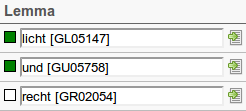
\includegraphics[width=0.28\textwidth]{img/lemma.png}\vspace{20px}
    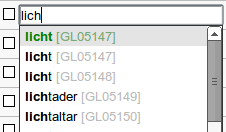
\includegraphics[width=0.28\textwidth]{img/lemma-edit.png}
  \end{center}
\end{wrapfigure}

Die Lemma-Spalte hat drei Bestandteile: eine \textbf{Checkbox}, um
Lemma-Einträge als "`bestätigt"' zu markieren; ein
\textbf{Eingabefeld} für das Lemma; und einen \textbf{Verweis} auf die
Online-Ausgabe des Grimmschen Wörterbuchs.

Das Eingabefeld ist mit einer \textbf{Dropdown-Liste mit
  Lemma-Vorschlägen} verknüpft.  Diese Liste öffnet sich automatisch,
sobald eine Eingabe in dem Feld gemacht wird (s.~Abbildung rechts).
Alternativ lässt sie sich auch durch Doppelklick in das Eingabefeld
oder mit "`Pfeiltaste nach unten"' öffnen.  Die Liste kann
verschiedene Arten von Einträgen enthalten:
\begin{enumerate}
\item \textbf{Grau hinterlegte} Einträge sind automatisch generierte
  Vorschläge.
\item Zusätzlich \textbf{grün hervorgehobene} Einträge sind Lemmata,
  die an anderer Stelle für eine gleichlautende Wortform bereits
  eingetragen und als "`bestätigt"' markiert wurden.  Diese Vorschläge
  werden aus allen Texten im selben Projekt generiert.  (Es ist
  allerdings erforderlich, dass die Lemma-Einträge bereits gespeichert
  wurden, damit sie für andere gleichlautende Wortformen als Vorschlag
  angezeigt werden können.)
\item Alle anderen Einträge sind durch Autovervollständigung gefundene Treffer im Grimmschen Wörterbuch. Dabei gilt:
  \begin{enumerate}
  \item es wird immer nur nach passendem Wortanfang gesucht;
  \item Diakritika in Grimm werden ignoriert, d.h.\ Eingabe von
    \emph{geta} findet sowohl \emph{getacht} wie auch \emph{getäckel}
    oder \emph{getâkel}; und
  \item wenn es sehr viele Treffer gibt, wird nur ein Teil davon
    angezeigt, d.h.\ befindet sich der gesuchte Eintrag nicht in der
    Liste, müssen Sie evtl.\ weitere Buchstaben dazu eingeben.
  \end{enumerate}
\end{enumerate}

Durch Anklicken eines Eintrags in der Liste wird dieser in das
Eingabefeld übernommen (alternativ: Auswählen mit den Pfeiltasten und
Drücken der "`Tabulator"'-Taste).  Das Textfeld akzeptiert aber auch
beliebige andere Eingaben; es muss nicht zwingend ein Eintrag aus der
Liste übernommen werden!

Die \textbf{Checkbox für "`bestätigte"' Lemmata} wird automatisch markiert,
wenn ein grün hervorgehobener Eintrag aus der Liste ausgewählt wird.
Ebenso wird eine Markierung automatisch wieder entfernt, wenn der
Lemma-Eintrag auf andere Weise geändert wird.  Dies soll vor
unabsichtlichen Fehlern (und damit vor falschen Einträgen, die
trotzdem "`bestätigt"' sind) schützen.

Klicken auf das
Symbol 
\includegraphics[height=\baselineskip]{img/lemma-link2.png}
öffnet die Online-Version des Grimmschen Wörterbuchs in einem
separaten Browserfenster.  Dabei wird automatisch der zu dem
eingetragenen Lemma passende Eintrag aufgerufen.  Weitere Aufrufe
öffnen sich immer in demselben Fenster.
% , sodass CorA- und
% Grimm-Browserfenster auch gut nebeneinander platziert werden können,
% wenn öfter in Grimm nachgeschlagen werden soll.

\subsubsection{Kommentarfeld}

Die Spalte "`Kommentar"' enthält ein Eingabefeld, worin ein beliebiger
Freitext eingegeben werden kann.  Diese Kommentare sind unabhängig von
Kommentaren in der Transkription (+K \ldots{}@K).

\subsubsection{Kontextmenü}

\vspace{-.5em} Klicken auf den
Pfeil 
\includegraphics[height=\baselineskip]{img/dropdown.png} öffnet
ein Kontextmenü.  Derzeit besteht es nur aus drei Einträgen, die sich
alle auf die Bearbeitung der Transkription beziehen, welcher der
Abschnitt~\ref{sec:bearbeiten} gewidmet ist.

\subsection{Horizontale Textansicht}
\label{sec:horizontal}

Am unteren Rand des Editors befindet sich eine Textansicht, die einen
Ausschnitt aus dem derzeit geöffneten Dokument wiedergibt.  Dort
können die Token nebeneinander (horizontal) statt untereinander
gelesen werden, um den Satzzusammenhang schneller zu erfassen.  Das
Token, das gerade annotiert wird, ist in dieser Ansicht gelb
hinterlegt (s.\ Abbildung~\ref{fig:horizontal}).  Diese Markierung
ändert sich immer dann, wenn ein Textfeld oder eine Dropdown-Box im
Editor angewählt bzw.\ bearbeitet wird.

Die horizontale Textansicht umfasst immer mindestens die Token, die
auf der aktuell angezeigten Seite sichtbar sind.  Nach Möglichkeit
erweitert CorA die Anzeige immer bis zu einer Satzgrenze, damit der
gesamte Satzzusammenhang gesehen werden kann.  Es gibt jedoch derzeit
ein Limit nach oben, wieviele Token als weiterer "`Kontext"' angezeigt
werden.

Aussehen und Inhalt der horizontalen Textansicht lassen sich z.~Zt.\
noch nicht näher konfigurieren; dies ist eventuell zu einem späteren
Zeitpunkt möglich.

\begin{figure}
  \centering
  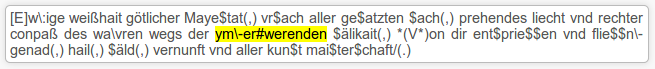
\includegraphics[width=0.8\linewidth]{img/textpreview.png}
  \caption{Horizontale Textansicht}
  \label{fig:horizontal}
\end{figure}


\subsection{Anpassen des Editors}
\label{sec:anpassen}

Das Aussehen des Editors kann in verschiedenen Punkten individuell
angepasst werden.

Die \textbf{Anordnung der Spalten} kann per "`Drag \& Drop"' geändert
werden.  Gehen Sie dazu auf eine beliebige Spalten-Überschrift,
klicken und halten Sie die linke Maustaste gedrückt, ziehen Sie die
Spalte an eine beliebige andere Position, und lassen die Maustaste
wieder los.  CorA merkt sich die individuelle Anordnung der Spalten
automatisch.

Weitere Anpassungen können \textbf{über den Reiter "`Einstellungen"'}
vorgenommen werden (s.\ Abbildung~\ref{fig:settings}).  Die
Einstellung \textbf{Zeilen pro Seite} steuert, wieviele Wortformen im
Editor gleichzeitig dargestellt werden.  Wir empfehlen, aus
Performance-Gründen nicht mehr als 50~Zeilen pro Seite anzeigen zu
lassen.  \textbf{Überlappende Zeilen} gibt an, wieviele Zeilen vom
Seitenende auch noch auf dem Anfang der nächsten Seite erscheinen
sollen.  Beide Einstellungen müssen durch Klick auf
"`Zeilen-Einstellungen übernehmen"' bestätigt werden.

Die Checkboxen unter \textbf{Sichtbare Spalten} steuern, welche
Spalten im Editor angezeigt werden.  Standardmäßig sind alle Spalten
sichtbar, durch Abwählen einzelner Checkboxen können bestimmte Spalten
jedoch ausgeblendet werden.  Dies kann der besseren Übersichtlichkeit
im Editor dienen.  Änderungen hier müssen nicht separat bestätigt
werden und sind sofort wirksam.

\begin{infobox}{Hinweis}
  Wenn Sie Spalten sichtbar machen, die zuvor ausgeblendet waren, kann
  es vereinzelt zu Darstellungsfehlern im Editor kommen.  Neuladen der
  Seite sollte dieses Problem beheben.  (Speichern Sie eventuelle
  Änderungen vorher ab!)
\end{infobox}

\begin{figure}
  \centering
  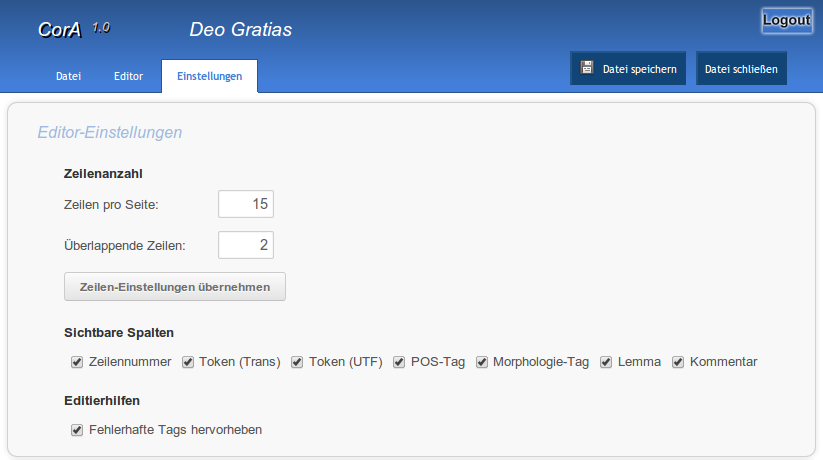
\includegraphics[width=\linewidth]{img/settings.png}
  \caption{Der Reiter "`Einstellungen"'}
  \label{fig:settings}
\end{figure}

Die Option \textbf{Fehlerhafte Tags hervorheben} steuert, ob
fehlerhafte Tags im Editor mit einer roten Umrandung versehen werden.

\newpage
\section{Bearbeiten der Transkription}
\label{sec:bearbeiten}

CorA ist in erster Linie ein Annotationstool, stellt jedoch auch
Funktionen für den Fall bereit, dass Änderungen an der
Original-Transkription vorgenommen werden müssen.  Die dafür nötige
Vorgehensweise kann anfangs -- je nach Art der Änderung --
möglicherweise etwas unintuitiv sein.  Dies ist zumeist dann der Fall,
wenn die Änderungen sich auf die Tokenisierung auswirken (z.B.\ wenn
zwei Wortformen, die in CorA auf zwei Zeilen verteilt sind,
zusammengezogen werden sollen).  Im Folgenden werden die einzelnen
Funktionen beschrieben und an einigen praktischen Beispielen
erläutert.

\begin{alertbox}{Wichtig!}
  \begin{itemize}\vspace{-1.5em}
  \item Vor jeder Änderung der Transkription müssen eventuell
    geänderte Annotationen \textbf{gespeichert} werden!
    Ungespeicherte Änderungen am Dokument gehen ansonsten verloren.
    (CorA weist Sie auch ggf.\ mit einem roten Hinweistext darauf
    hin.)
  \item Änderungen an der Transkription sind augenblicklich
    gespeichert und können \textbf{nicht rückgängig} gemacht werden!
    Sie können die Transkription zwar per Hand wieder zurück ändern,
    es gibt jedoch keine Möglichkeit, den Zustand der Transkription
    vor der Bearbeitung zu sehen.
  \end{itemize}
\end{alertbox}

Durch Klick auf das
Symbol 
\includegraphics[height=\baselineskip]{img/dropdown.png}
(standardmäßig ganz am Ende jeder Zeile) öffnet sich ein Kontextmenü,
worüber alle Funktionen zum Ändern der Transkription aufgerufen werden
können:

\begin{center}
  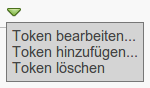
\includegraphics[width=0.25\linewidth]{img/dropdown-menu.png}
\end{center}

Die Funktion "`Token bearbeiten"' kann außerdem aufgerufen werden
durch \textbf{Doppelklick} auf die entsprechende Wortform in der
Spalte "`Token~(Trans)"' oder "`Token~(UTF)"'.

\subsection{Token bearbeiten}
\label{sec:trans-edit}

\begin{figure}
  \centering
  \begin{subfigure}[b]{0.4\textwidth}
    \centering
    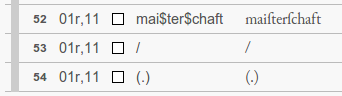
\includegraphics[width=\textwidth]{img/trans-bsp1.png}
    \caption{}
    \label{fig:trans-bsp1}
  \end{subfigure}
  \hfill
  \begin{subfigure}[b]{0.5\textwidth}
    \centering
    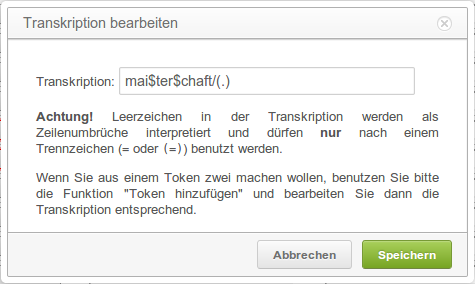
\includegraphics[width=\textwidth]{img/trans-edit1.png}
    \caption{}
    \label{fig:trans-edit1}
  \end{subfigure}
  \caption{Bearbeiten der Original-Transkription}
  \label{fig:trans-edit}
\end{figure}

Für die Bearbeitung der Transkription ist es wichtig zu verstehen,
dass die Zeilen im Editor und die Transkription, die bearbeitet wird,
sich nicht immer 1:1 entsprechen.  Dies lässt sich am besten an einem
Beispiel erläutern: Abbildung~\ref{fig:trans-bsp1} zeigt einen
Ausschnitt von drei Zeilen aus dem Editor;
Abbildung~\ref{fig:trans-edit1} zeigt das Fenster, das sich öffnet,
wenn eine beliebige dieser drei Zeilen bearbeitet wird.  Die
Transkription \trans{mai\$ter\$chaft/(.)} wird für die Annotation in
die drei separaten Token \trans{mai\$ter\$chaft}, \trans{/} und
\trans{(.)} zerlegt, während die Bearbeitung dieser Transkription
jedoch als Ganzes erfolgt.

Im Editorfenster aus Abbildung~\ref{fig:trans-edit1} können nun
beliebige Änderungen vorgenommen werden, die nach einem Klick auf
"`Speichern"' übernommen werden.  Für alle Änderungen gilt, dass diese
zunächst mit Hilfe des Check-Skripts geprüft werden.  Ungültige
Transkriptionszeichen werden von CorA nicht akzeptiert; die
entsprechende Fehlermeldung des Check-Skripts wird dann angezeigt und
die Änderung wird nicht vorgenommen.

\textbf{Leerzeichen in der Transkription} haben an dieser Stelle eine
besondere Bedeutung.  Sie werden von CorA immer dann verwendet, wenn
sich ein Token in der Original-Transkription über mehrere Zeilen
erstreckt:

\begin{quote}\ttfamily\small
  F137-02r,20~~~~dein hoche vernunft \$o begirlich be=\\
  F137-02r,21~~~~gert(,) \$u\*cht vnd erfra\textbackslash{}vgt(,) alle kun\$t
\end{quote}

Das Token, das sich hier über beide Zeilen erstreckt, würde beim
Bearbeiten in CorA als \trans{be=~gert(,)} angezeigt.  Das Leerzeichen
markiert dabei die Stelle, an der der Zeilenumbruch stattfindet.
Dieses Leerzeichen darf beim Bearbeiten der Transkription nicht
entfernt werden, da ansonsten der hintere Teil in der
Original-Transkription mit auf die vorherige Zeile gezogen würde!

Andersherum dürfen Leerzeichen beim Bearbeiten der Transkription nur
dann eingefügt werden, wenn Sie einen Zeilenumbruch repräsentieren
sollen.  Dies ist nur möglich, wenn das bearbeitete Token am Ende
einer Zeile steht und wird ansonsten von CorA nicht akzeptiert.
Außerdem muss jedem Leerzeichen ein Trennzeichen vorausgehen.

\begin{infobox}{Tipp}
  Möchten Sie einmal in die Transkription tatsächlich ein Leerzeichen
  einfügen, das nicht für einen Zeilenumbruch steht (z.B.\ um
  \trans{in\#der} in \trans{in der} abzuändern), so sind dafür mehrere
  Schritte nötig!  In Abschnitt~\ref{sec:trans-bsp} wird dies an
  Beispielen verdeutlicht.
\end{infobox}

\subsection{Token hinzufügen}

\begin{figure}
  \centering
  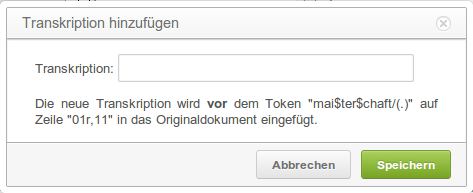
\includegraphics[width=0.6\linewidth]{img/trans-add.png}
  \caption{Hinzufügen eines Tokens}
  \label{fig:trans-add}
\end{figure}

Wählen Sie "`Token hinzufügen\ldots"' aus dem Kontextmenü aus, um eine
neue Transkription \textbf{vor} einem bestehenden Token einzufügen.
Es öffnet sich ein Fenster, worin die neue Transkription eingegeben
werden kann (s.\ Abbildung~\ref{fig:trans-add}).  Dabei gelten
dieselben Regeln wie für das Bearbeiten einer Transkription (siehe
oben); insbesondere darf die Transkription kein Leerzeichen enthalten.

In einem Hinweistext unter dem Eingabefeld wird nochmals erläutert, an
welcher Position und auf welcher Zeile der Original-Transkription das
neue Token eingefügt wird.  Überprüfen Sie diese Angaben in jedem
Fall, um sicherzustellen, dass Sie das Token an der richtigen Stelle
im Text einfügen!

\subsection{Token löschen}

Wählen Sie "`Token löschen"' aus dem Kontextmenü aus, um eine
Transkription komplett aus dem Text zu löschen.  Sie müssen diese
Aktion zur Sicherheit immer bestätigen, da auch das Löschen eines
Tokens nicht rückgängig gemacht werden kann.  In dem entsprechenden
Hinweisfenster können Sie außerdem nochmals überprüfen, welche
Transkription bei einem Bestätigen der Aktion tatsächlich gelöscht
wird.

\subsection{Praktische Beispiele}
\label{sec:trans-bsp}

Für Änderungen in der Transkription, die Einfluss auf die
Tokenisierung haben, können mitunter mehrere Bearbeitungsschritte
notwendig sein.  Daher werden hier einige Beispiele gegeben, wie die
Transkription in diesen Fällen geändert werden kann.

\paragraph{Beispiel 1.}  Angenommen, ein Token in der Transkription
soll (durch Einfügen eines Leerzeichens) in zwei Token aufgetrennt
werden.  Ein Beispiel wäre die Änderung von \trans{in\#der} zu
\trans{in der}.  Hierzu sind zwei Schritte nötig:
\begin{enumerate}
\item Gehen Sie auf die Zeile mit der Transkription \trans{in\#der},
  öffnen Sie das Kontextmenü
  (
\includegraphics[height=\baselineskip]{img/dropdown.png}), und
  wählen Sie "`Token hinzufügen"'.  Fügen Sie jetzt \trans{in} als
  neue Transkription ein.\\$\to$ In der Transkription steht jetzt
  \trans{in in\#der}.
\item Doppelklicken Sie nun auf die Transkription \trans{in\#der} und
  ändern Sie sie ab zu \trans{der}.\\$\to$ In der Transkription steht
  jetzt \trans{in der}.
\end{enumerate}

\paragraph{Beispiel 2.}  Angenommen, zwei Token in der Transkription
sollen zu einem zusammengefügt werden.  Beispielsweise soll
\trans{zu~vor} geändert werden in \trans{zu\#vor}.  Dies ist der
umgekehrte Fall zu Beispiel~1.  Hierfür sind ebenfalls wieder zwei
Schritte nötig:
\begin{enumerate}
\item Doppelklicken Sie auf die Transkription \trans{vor} und ändern
  Sie sie ab zu \trans{zu\#vor}.\\$\to$ In der Transkription steht
  jetzt \trans{zu~zu\#vor}.
\item Gehen Sie nun auf die Zeile mit der Transkription \trans{zu},
  öffnen Sie das Kontextmenü, und wählen Sie "`Token löschen"'.\\$\to$
  In der Transkription steht jetzt \trans{zu\#vor}.
\end{enumerate}

\begin{infobox}{Tipp}
  Seien Sie besonders vorsichtig, wenn sie eine Transkription
  bearbeiten, die sich über mehrere Zeilen erstreckt!  Angenommen, in
  der folgenden Original-Transkription sollen die ersten beiden Token
  zu \trans{MVLLNER\#ORD=~nung} zusammengefügt werden:

  \begin{quote}\ttfamily\small
    F57-1r,01~~~~MVLLNER ORD=\\
    F57-1r,02~~~~nung in den Für\$tlichen Thiroli\$chen Stet=
  \end{quote}

  Dies kann wie oben beschrieben erreicht werden, indem Sie in CorA
  zunächst das Token \trans{ORD=~nung} abändern in
  \trans{MVLLNER\#ORD=~nung}, und anschließend das erste Token
  \trans{MVLLNER} löschen.

  Andersherum ist es jedoch \textbf{nicht} möglich, zuerst
  \trans{MVLLNER} in \trans{MVLLNER\#ORD=~nung} zu ändern und dann das
  Folgetoken zu löschen!  Die entsprechende Operation wird
  fehlschlagen, da die neue Transkription ein Leerzeichen
  (=~Zeilenumbruch) enthält, das Token \trans{MVLLNER} sich jedoch
  nicht am Zeilenende befindet.

  Behelfen Sie sich \textbf{in keinem Fall}, indem Sie das Leerzeichen
  weglassen oder entfernen!  Das Ergebnis würde dann fälschlicherweise
  so interpretiert\ldots{}

  \begin{quote}\ttfamily\small
    F57-1r,01~~~~MVLLNER\#ORD=nung\\
    F57-1r,02~~~~in den Für\$tlichen Thiroli\$chen Stet=
  \end{quote}

  \ldots{}was vermutlich nicht Ihrer Absicht entspricht.
\end{infobox}

\paragraph{Beispiel 3.}  Angenommen, ein fälschlich gesetztes
Trennzeichen am Zeilenende soll entfernt werden.  Beispielsweise soll
\trans{in(=)~der} zu \trans{in~der} geändert werden, wobei die beiden
Wortformen auf verschiedenen Zeilen in der Transkription stehen.  Dies
kann mit folgenden Schritten realisiert werden:
\begin{enumerate}
\item Gehen Sie auf die erste Zeile \textbf{nach} der Transkription
  \trans{in(=)~der}, öffnen Sie das Kontextmenü, und wählen Sie
  "`Token hinzufügen"'.  Fügen Sie jetzt \trans{der} als neue
  Transkription ein.\\$\to$ In der Transkription steht jetzt
  \trans{in(=)~der~der}.
\item Doppelklicken Sie nun auf die Transkription \trans{in(=)~der}
  und ändern Sie sie zu \trans{in}.\\$\to$ In der Transkription steht
  jetzt \trans{in~der}.
\end{enumerate}

\paragraph{Beispiel 4.}  Angenommen, das Token \trans{ge} am Ende
einer Zeile soll mit dem ersten Token \trans{schah} der nächsten Zeile
mittels eines Trennstriches \trans{(=)} zusammengeführt werden.  Dies
gelingt mit folgenden Schritten:
\begin{enumerate}
\item Doppelklicken Sie auf die Transkription \trans{ge} und ändern
  Sie sie zu \trans{ge(=)~schah} (Leerzeichen beachten!).
\item Löschen Sie nun einfach das zweite \trans{schah}.
\end{enumerate}

\vspace{2em} %% HACK
\section{Tastaturbefehle}

Im Folgenden werden einige Tastaturbefehle aufgeführt, die für ein
zügigeres Arbeiten in CorA hilfreich sein können.  Diese Liste wird im
Laufe der Zeit noch ergänzt.

Mit \textbf{Tab} (Tabulator-Taste) springen Sie im Editor zum nächsten
editierbaren Feld, mit \textbf{Shift+Tab} springen Sie ein Feld
zurück.  (Dies ist eine Funktion Ihres Internetbrowsers, nicht von
CorA selbst.)

In den Dropdown-Menüs für POS- und Morphologie-Tags können Sie mit
\textbf{Pfeiltaste nach oben/unten} zwischen den Tags wechseln.
Dasselbe gilt für das Menü mit den Lemma-Vorschlägen.  Alternativ
können Sie auch die Anfangsbuchstaben des gewünschten Tags eingeben.
(Dies ist eine Funktion Ihres Internetbrowsers, nicht von CorA
selbst.)

Mit \textbf{Strg+S} können Sie die aktuelle Datei speichern.

\newpage
\section{Umgang mit Fehlermeldungen}
\label{sec:error}

\begin{figure}
  \centering
  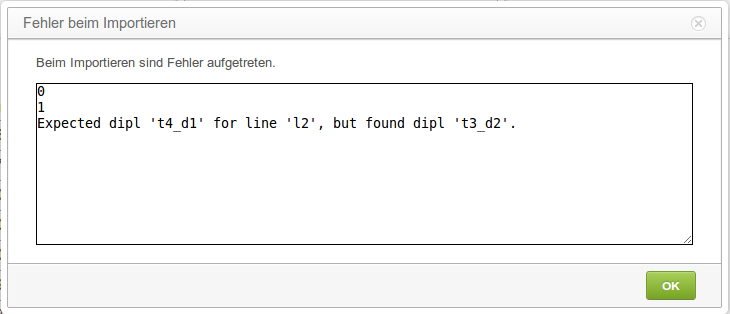
\includegraphics[width=0.8\linewidth]{img/import-error.png}
  \caption{Eine Fehlermeldung beim Import}
  \label{fig:import-error}
\end{figure}

Trotz aller Bemühungen können wir leider nicht ganz ausschließen, dass
während der Benutzung von CorA auch Fehlermeldungen auftreten.  In
unvorhergesehenen Fällen können diese Meldungen mitunter recht
kryptisch sein; Abbildung~\ref{fig:import-error} zeigt ein Beispiel
für eine (hoffentlich niemals auftretende\ldots) Fehlermeldung beim
Importieren einer Datei.  Damit wir in so einem Fall das
zugrundeliegende Problem so schnell wie möglich beheben können, bitten
wir Sie darum, ein paar einfache Hinweise zu beachten.

\begin{enumerate}
\item Melden Sie Fehler immer per \textbf{E-Mail} an \mmb{}.
\item Melden Sie uns Fehler, die Sie sich nicht erklären können, bitte
  in jedem Fall!  Wir können nur Fehler beheben, von denen wir auch
  wissen.
\item Senden Sie uns eine \textbf{aussagekräftige} Beschreibung des
  Fehlers! Dazu sollten immer folgende Informationen gehören:
  \begin{itemize}
  \item Was genau haben Sie unmittelbar vor dem Auftreten des Fehlers
    getan? (z.B.\ \emph{auf den Knopf "`Datei speichern"' geklickt})
  \item Wie genau äußert sich der Fehler? Falls es eine Fehlermeldung
    gibt: bitte die komplette Meldung kopieren und einfügen!
  \item An welcher Datei oder welchem Token genau haben Sie
    gearbeitet, als der Fehler auftrat? Falls der Fehler beim
    Importieren auftritt: die Datei, die importiert werden sollte, als
    Anhang mitschicken!
  \end{itemize}
\end{enumerate}

\end{document}
